\documentclass[10pt,conference,compsocconf]{IEEEtran}

%\usepackage{times}
%\usepackage{balance}
\usepackage{url, amsmath, amssymb}
\usepackage{graphicx}    % For figure environment
\usepackage{textcomp}
\usepackage{amsfonts}
\usepackage[ruled,vlined]{algorithm2e}

\usepackage[hidelinks,bookmarksnumbered,unicode]{hyperref} % Enables cross linking in the electronic document version. This package has to be included second to last.
\usepackage[noabbrev,nameinlink]{cleveref}
\usepackage{balance}
\usepackage{nag}       % Issues warnings when best practices in writing LaTeX documents are violated.
\usepackage{booktabs}
\usepackage{amsmath}   % Improves the typesettings of tables.


\newcommand{\spacing}{\hspace{1cm}}
\begin{document}
    \title{Collaborative Filtering}

    \author{
        Rafael Sterzinger \spacing Patrik Okanovic \spacing Fatjon Zogaj \spacing Filip Batur Stipic\\
        Group: Terminators\\
        Department of Computer Science, ETH Zurich, Switzerland
    }

    \maketitle

    \begin{abstract}

    \end{abstract}


    \section{Introduction}

    The goal of designing Recommender Systems is to recommend the item most likely to be of interest to a target user based on past data.
    Collaborative Filtering is one of the standard computational methods that attempts to solve this problem by leveraging the similarities between users and items in some vector space \cite{CF_survey}.
    Usually, the preference data of users to items is represented by a real-valued sparse matrix, given that the majority of users does not rate most movies.
    In this project we are concerned with completing such sparse matrices, in which each observed entry represents the rating of a user for some movie.


    In the past two decades, the community had been concerned with constructing benchmarks for different recommendation tasks as well as using novel machine learning techniques in order to tackle the problem in a controlled fashion and in ever more elaborate ways.
    Some of the most famous benchmarks whose data also represents movie ratings are the Netflix Prize \cite{Netflix} and MovieLens \cite{Movielens}.
    The most well-established baselines for these benchmarks include Matrix Factorization models, such as Singular Value Decomposition \cite{svd}, Alternating Least-Squares \cite{als} and Bayesian Factorization Machines and its variants \cite{freudenthaler_bayesian_2011, salakhutdinov_bayesian_2008}.
    The core idea behind such models is that preferences of users over movies are only determined by a small number of unobserved factors.
    These latent factors are assumed to be feature vectors for each user and movie separately, so that the corresponding rating of a user for a movie is represented by a dot product between the latent feature vector for that particular user and movie (...)

    Some of the more recent, neural-based successful approaches include: Neural Collaborative Filtering \cite{DBLP:journals/corr/abs-1708-05031}, Autoencoders for Collaborative Filtering \cite{inproceedings} and Neural Graph Collaborative Filtering \cite{ngcf}.

    Surprisingly enough, the now seminal paper: "On the Difficulty of Evaluating Baselines" by Rendle et al. \cite{rendle_difficulty_2019} showed that by carefully tuning the existing simple baselines by doing more extensive hyperparameter searches, the performance of the baselines can be drastically improved.
    Most notably, the authors demonstrate that Bayesian Factorization Machines \cite{freudenthaler_bayesian_2011, salakhutdinov_bayesian_2008} when used in conjunction with the common initialization technique SVD++ \cite{koren_factorization_2008} can outperform any result on the MovieLens benchmark up to date.

    Since, Graph Neural Networks had especially surged in popularity, and most very recent papers in Collaborative Filtering for Recommendation Systems attempt to exploit their alleged ability to model topologically richer dependencies between users and items, one way or another.
    However, since GNN based approaches for Collaborative filtering had still not been shown to systematically beat the afore mentioned Bayesian FM for movie recommendation benchmarks \cite{gnn_survey}, we choose rather to focus on improving the current state-of-the-art Bayesian Factorization Machine by ...


    \section{Models and Methods}
    In the following section we describe the different methods we used combined with our baselines and our final best model.

    %TODO if done de-biasing

    \subsection{Preprocessing: Missing Values Initialization}
    As the majority of our models depends on the whole data matrix as input, we experiment with a variety of initialization techniques for the unobserved/missing values.
    Our approaches include replacement by the total mean, user mean and item mean of rankings.
    We add upon this by enabling a model to be used for predicting the missing values that then get used in another model.
    This also allows us to iteratively chain multiple models to predict the unobserved values for the respective following one.

    \subsection{Postprocessing: Clipping}
    As a final step after the prediction we try out various ways to postprocess the output.
    The default way is a simple clipping between 1 and 5.
    As the rankings are given as integers, values such as 1.15 do not make a lot of sense.
    A prediction of the model to be closer to 1 than 2, leads to an "unnecessary" error when it guesses correctly, but outputs real values.
    We try rounding the outputs to the nearest integer as well as to the nearest quarter (.00, .25, .50, .75).

    \subsection{Singular Value Decomposition}

    \subsection{Non-Negative Matrix Factorization}

    \subsection{Autoencoder}
    An autoencoder is a neural network that is trained to attempt to copy its input to its output.
    Internally, it has a hidden layer $\textbf{h} \in \mathbb{R}^k$ that describes a code used to represent the input.
    The network may be viewed as consisting of two parts: an encoder function $f: \mathbb{R} ^d \rightarrow \mathbb{R} ^k$ and a
    decoder that produces a reconstruction $g: \mathbb{R} ^k \rightarrow \mathbb{R} ^d$ \cite{Goodfellow-et-al-2016}. Autoencoders
    have proven to achieve good results in collaborative filtering \cite{inproceedings}. We examine the user-based
    autoencoder as opposed to item-based autoencoder which achieved a good score in \cite{inproceedings}. Both encoder
    and decoder consist of feedforward neural networks with ReLU activation functions. We train the model by minimizing
    the squared reconstruction loss. Important part of the implementation is the fact that inputs are partially observed
    and therefore we only update those weights that are associated with observed inputs during backpropagation.
    We found that when both encoder and decoder consist of one layer increasing the encoded dimension up to 500 makes
    the score better. Furthermore, we have examined the effect of compositionality. Using only two layers in encoder
    and decoder already performs better than any single layer autoencoder.

    \subsection{Neural Collaborative Filtering}
    Neural Collaborative Filtering approach as proposed by He et al. \cite{DBLP:journals/corr/abs-1708-05031}, tries to
    jointly learn user-item latent representations as well as the prediction depending on the interactions between
    different users and items. The network's inputs are indices of users and items. Firstly, an embedding layer maps
    each user and each item to its corresponding latent vector representation. Output of the embedding layers is then
    concatenated and passed on through fully connected feedforward layers with ReLU activation functions. Finally,
    output of the network represents the rating associated with the inputted user and item. Network is trained minimizing
    the mean squared error loss between the predicted and target rating. TODO: erase? Further, improvements would be
    implementing the network as a classification task between the movie rating rather then regressing the predicted rating.

    \subsection{Kernel Net}
    We add the MovieLens-1M state of the art model (on papers with code) as another baseline as the given problem description fares very similarly to ours.
    For this, we adapt the code from \cite{pmlr-v80-muller18a, kernelNetGithub} into our experiment framework.

    The high sparsity in recommender-system datasets leads to the need and resulting variety of possibilities for dimensionality reduction.
    Combined with the amount of parameters in neural networks this leads to large training times and possibly
    unexpected results on unseen data due to overfitting.

    Muller et al. make use of finite-support kernels to reparametrize weight matrices with low-dimensional vectors.
    This allows for the structured feature embedding of neural network weights based on the specific kernel function used and
    acts as regularization.
    As such, their item-based autoencoder is able to reduce complexity at inference time while improving performance compared to similar models.\cite{pmlr-v80-muller18a}


    %\citeauthor{pmlr-v80-muller18a}

    \subsection{Bayesian Factorization Machines}
    For our final baseline, we explored Bayesian Factorization Machines \textbf{(BFM)} which are Bayesian variants of the former known Factorization Machines \textbf{(FM)} \cite{rendle_factorization_2010}.
    In its core, FMs build upon the advantages of Support Vector Machines \textbf{(SVM)} but use a factorized parametrization instead of a dense one.
    With this parametrization, FMs are able to estimate all possible interactions between entries of $\mathbf{X}$ even in setting where the data matrix $\mathbf{X}$ is highly sparse.
    Similarly to SVMs with a polynomial kernel, the FM model equation which captures all single and pairwise interactions, can be formulated as follows:

    $$\hat{y}(\mathbf{x})=w_0+\sum^n_{i=1}w_ix_i + \sum^n_{i=1}\sum^n_{j=i+1}\langle \mathbf{v_i},\mathbf{v_j} \rangle x_ix_j$$

    Here, $v_i$ denotes a vector in $\mathbb{R}^k$ which describes the $i$-th variable with $k$ dimensions and $\langle \mathbf{v_i},\mathbf{v_j} \rangle$ the interaction between the variables $i$ and $j$.
    Instead of using a fixed weight $w_{ij}$, this factorization via the dot product allows FMs to predict parameters for related interaction, e.g. different users but same movie.
    In the non-Bayesian setting, model parameters are optimized with stochastic gradient descent.
    Opposed to this are Bayesian variants of FMs where model parameters are estimated via maximum a posteriori estimation by means of Markov Chain Monte Carlo methods for approximate inference \cite{salakhutdinov_bayesian_2008}.
    This fully Bayesian treatment of FMs does not only increase the accuracy of such a model but also omits the need of exhaustive parameter tuning \cite{freudenthaler_bayesian_2011}.
    Regarding, the implementation of our baseline, we utilize a package named \textit{myFM} \cite{noauthor_myfm_nodate} which employs Gibbs sampling for approximate inference of the posterior.
    Besides this standard variant of BFMs, multiple additions have been made by means of exploiting additional implicit information about users, items, and temporal dynamics \cite{rendle_scaling_2013,koren_factorization_2008,koren_collaborative_2009}.
    In our implementation, we incorporated most of these as well, omitting temporal dynamics due to the absence of this information in our provided dataset.
    The two additional features are defined as follows:
    \begin{enumerate}
        \item Implicit User Feature (Bayesian SVD++) $\Leftrightarrow$ all items consumed by user $u$:
        $$\mathbf{V}_u=\frac{\Omega_u}{\sqrt{|\{(u,i): (u,i) \in \Omega_u\}|}}$$
        \item Implicit Item Feature (Bayesian SVD++ flipped) $\Leftrightarrow$ all users that consumed item $i$:
        $$\mathbf{W}_i=\frac{\Omega^T_i}{\sqrt{|\{(u,i): (u,i) \in \Omega^T_i\}|}}$$
    \end{enumerate}
    After one-hot-encoding users $\mathbf{U}$ and items $\mathbf{I}$, denoted as the identity matrix $I_k$ with corresponding dimension $k$, a single entry in our dataset would have the following form:
    $$\mathbf{x}_{ui} = [(I_n)_u,\mathbf{V}_u,(I_m)_i,\mathbf{W}_i, r_{ui}]$$

    Additionally, datasets commonly used in the setting of collaborative filtering such as the MovieLens dataset include much more detailed information on users/items.
    In the setting of movie recommendations, for instance, the genre or the release date of a movie, a timestamp of when the user gave the rating, or user specific information such as who is friends with whom might be included.
    As we found that these details might be greatly beneficial for our prediction task, we created features which resemble the previously mentioned ones based on the limited data we were provided.
    Here, we concentrated mainly on two aspects, calculating the similarity between users to imitate the "friends of a user" feature, and clustering a movie embedding space to create a "movie genre" feature.

    \subsubsection{User Features}
    Regarding the additional user features in the form of similarity measures between two users, we looked at different variants of the Jaccard index, the standard variant and an improved version of it \cite{lee_improving_2017}.
    The standard Jaccard index measures the similarity between two users u and v as follows:
    $$\text{Jac}(u,v)=\frac{|\mathbf{I}_u \cap \mathbf{I}_v|}{|\mathbf{I}_u \cup \mathbf{I}_v|}$$
    Furthermore, we experimented with an improved version of the Jaccard index.
    Here, the set of items $\mathbf{I}_u$ a user $u$ has consumed is subdivided into three parts $L,M,$ and $H$ with two boundaries $L_{bd}$ and $H_{bd}$.
    Given these boundaries the sets are formulated as follows:
    \begin{align*}
        &\mathbf{I}_{L,u}=\{i \in \mathbf{I}_u : r_{u,i} \leq L_{bd}\}\\
        &\mathbf{I}_{M,u}=\{i \in \mathbf{I}_u : L_{bd} < r_{u,i} < H_{bd}\}\\
        &\mathbf{I}_{H,u}=\{i \in \mathbf{I}_u : H_{bd} \leq r_{u,i}\}\\
    \end{align*}
    The improved Jaccard index with these definied subsets is denoted as follows:
    $$\text{Jac}_{LMH}=\frac{1}{3}(\text{Jac}_L(u,v) + \text{Jac}_M(u,v) + \text{Jac}_H(u,v))$$
    According to the authors the bound $L_{bd} = 3$ and $H_{bd}=4$ yielded the best results on the MovieLens dataset.
    As such, we set the same bounds, effectively splitting into two instead of three sets.

    \subsubsection{Movie Features}
    In order to provide additional information for models, we implement clustering and that way provide the information
    about movie categories as in the MovieLens dataset. First we initialize the matrix using FM:TODO.
    Afterwards, we perform Singular Value Decomposition with the rank that showed best results (TODO ref the plot).
    We get the embeddings using the following expression: assuming $A=U\Sigma V^T$ then the matrix corresponding to the movie embeddings is equal to $\Sigma _k ^{\frac{1}{2}} V_k ^T$.
    Finally, after obtaining the k-rank movie embeddings we search for the optimal number of clusters in K-Means clustering.
    We visualize the clusters in 2 dimensions. Since, visualizing in two dimensions does not easily distinct the optimal
    number of clusters we choose 18 as in the MovieLens dataset as the number of clusters. \Cref{fig:movie_category_distribution}
    shows two peaks in movie categories while other categories look uniformly distributed.

    \begin{figure}
        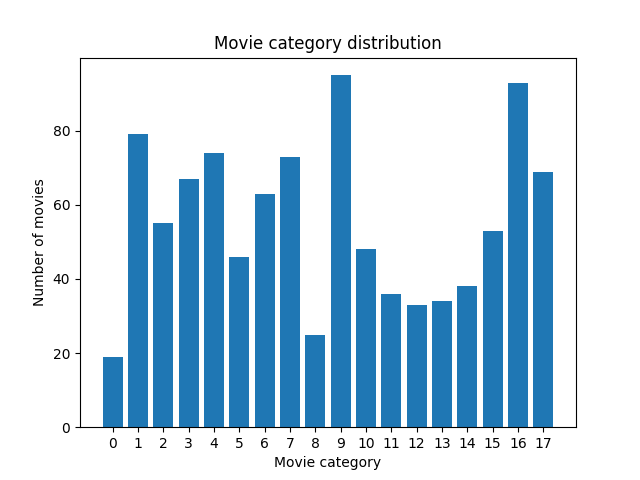
\includegraphics[width=\columnwidth]{figures/movie_category_distribution.png}
        \caption{Distribution of movie categories between 18 categories as in MovieLens dataset.}
        \label{fig:movie_category_distribution}
    \end{figure}

    With these additional user/item features, we append to our feature vector $\mathbf{x}_{ui}$ a dense vector of user similarities from user $u$ to every other user, or the item feature which is either the one-hot-encoded cluster of item $i$ or a dense vector of Euclidean/Mahalanobis distances from item $i$ to every other item.

    Finally, the following \Cref{alg:algo1} shows our proposed procedure for creating additional features to run \textbf{BFM}

    \begin{algorithm}
        \SetKwInOut{Input}{input}
        Initialize missing matrix value with FM\\
        \For{$k = 0...K$} {
            Run SVD (rank=$k$)
            $k_{opt}=argmin_{k, k_{opt}}$RMSE(SVD(rank=$k$))
        }
        Movie embeddings= $\sqrt{\Sigma_{k_{opt}}}V_{k_{opt}}^T$\\
        Perform K-Means(movie embeddings)\\
        \For{$i = 0...numMovies$} {
            \For{$j = 0...numMovies$} {
                $D_{i,j} ^{Eucl} = \|embi - emb_j\|^2$
            }
        }
        \For{$i = 0...numMovies$} {
            \For{$j = 0...numMovies$} {
                $D_{i,j} ^{Mahal} = \sqrt{(emb_i-emb_j)^TCov^{-1}(emb_i-emb_j)}$
            }
        }
        \caption{Proposed solution for collaborative filtering}
        \label{alg:algo1}
    \end{algorithm}

    \subsubsection{Iterative SVD}
    % maybe only have in results?
    % TODO: run from 1-10, 20-100

    \subsubsection{Ensembles}


    \section{Results and Discussion}
    We present our results in \Cref{tab:ablation}, noting the Root Mean Squared Error (RMSE) of our baselines and final model.
    Test scores refer to the public leaderboard ranking while validation scores refer to a 10\% holdout of our training data.
    Models without test scores did not perform well enough and were thus only evaluated on the validation dataset.
    Some other models may only show test scores, e.g. if they were directly evaluated on the test data to eliminate
    fitting the model twice (once on 90\% of training data and then on all the training data).

    \begin{table}
        \centering
        \resizebox{\columnwidth}{!}{
            \begin{tabular}{|| c | c | c | c | c ||}
                \hline
                \textbf{Model} & \textbf{Params}                   & \textbf{ Init Missing } & \textbf{RMSE}$_{test}$ & \textbf{RMSE}$_{valid}$ \\
                \hline
                SVD            & Singular Values 2                 & total mean              & 1.07131                &                         \\
                SVD            & Singular Values 2                 & user mean               & 1.05584                &                         \\
                SVD            & Singular Values 2                 & item mean               & 1.01375                &                         \\
                SVD*4          & Singular Values 2                 & item mean               & 0.99306                &                         \\
                SVD*7          & Singular Values 2                 & item mean               & 0.99123                &                         \\
                SVD*10         & Singular Values 2                 & item mean               & 0.98817                & 0.98540                 \\
                SVD*10         & Singular Values 2, Round Quarters & item mean               & 0.99071                &                         \\
                \hline
                NMF            & Singular Values 2                 & total mean              & 1.01375                &                         \\
                \hline
                KernelNet      & 50 Iterations                     & zero                    & 1.00031                &                         \\
                KernelNet      & 150 Iterations                    & zero                    & 0.98603                &                         \\
                KernelNet      & 300 Iterations                    & zero                    & 0.98894                &                         \\
                KernelNet      & 450 Iterations                    & zero                    & 0.98860                &                         \\
                \hline
                BFM            & Jaccard Similarity                & /                       & 0.96940                &                         \\
                BFM            & Improved Jacc. Sim.               & /                       & 0.99742                &                         \\
                BFM            & Ordered Probits                   & /                       & \textbf{ 0.96572 }     &                         \\
                BFM            & Ordered Probits, Round Quarter    & /                       & 0.96842                &                         \\
                \hline
            \end{tabular}
        }
        \caption{We note Root Mean Squared Error (RMSE) on test and validation datasets to compare our baselines.
        Arithmetic in models such as $x * 4$ or $x + y$ refers to the iterative chaining of multiple models for the initialization of missing values.
        }
        \label{tab:ablation}
    \end{table}

    \subsection{Comparison to Baselines}

    You compare your novel algorithm to \emph{at least two baseline
    algorithms}. For the baselines, you can use the implementations you
    developed as part of the programming assignments.


    \section{Conclusion}

    Organize the results section based on the sequence of table and
    figures you include. Prepare the tables and figures as soon as all
    the data are analyzed and arrange them in the sequence that best
    presents your findings in a logical way. A good strategy is to note,
    on a draft of each table or figure, the one or two key results you
    want to address in the text portion of the results.
    The information from the figures is
    summarized in Table.




    \balance
    \bibliographystyle{IEEEtran}
    \bibliography{bibliography}
\end{document}
